\documentclass[11pt]{article}

% ---------------------------------------------------------------------------
% AEGIS-AT v2 --- Attribution Integrity Benchmark
% Self-contained, arXiv-ready LaTeX source.
% Compiles with pdflatex (run twice for cross-references / hyperref).
% Figures are generated by figures/make_figures.py (run it first); they are
% produced from the live harness, so the plotted numbers cannot drift from
% the code. Dependencies are standard TeX Live / MiKTeX packages.
% ---------------------------------------------------------------------------

\usepackage[utf8]{inputenc}
\usepackage[T1]{fontenc}
\usepackage[margin=1in]{geometry}
\usepackage{amsmath,amssymb}
\usepackage{booktabs}
\usepackage{xcolor}
\usepackage{microtype}
\usepackage{caption}
\usepackage{enumitem}
\usepackage{listings}
\usepackage{lmodern}
\usepackage{graphicx}
\graphicspath{{figures/}}
\usepackage[hidelinks]{hyperref}
\hypersetup{
  colorlinks=true,
  linkcolor=black,
  citecolor=black,
  urlcolor=blue!55!black,
  pdftitle={AEGIS-AT v2: Does Sender-Constraint Recover Attribution? DPoP, Chain Depth, and a Log-Integrity Metric},
  pdfauthor={Rahul Singh}
}

% Code listing style ---------------------------------------------------------
\definecolor{codebg}{gray}{0.96}
\definecolor{codecomment}{rgb}{0.30,0.45,0.30}
\definecolor{codekw}{rgb}{0.20,0.20,0.60}
\lstdefinestyle{aegis}{
  basicstyle=\ttfamily\footnotesize,
  backgroundcolor=\color{codebg},
  commentstyle=\color{codecomment}\itshape,
  keywordstyle=\color{codekw}\bfseries,
  numbers=none,
  frame=single,
  framesep=4pt,
  rulecolor=\color{gray!40},
  breaklines=true,
  showstringspaces=false,
  captionpos=b,
  xleftmargin=4pt,
  xrightmargin=4pt
}
\lstset{style=aegis}

% Convenience macros ---------------------------------------------------------
\newcommand{\ais}{\textsc{ais}}
\newcommand{\lis}{\textsc{lis}}
\newcommand{\code}[1]{\texttt{#1}}
\newcommand{\actsub}{\code{act.sub}}
\newcommand{\cnf}{\code{cnf}}
\newcommand{\jkt}{\code{jkt}}
\newcommand{\siem}{\code{siem\_action}}
\newcommand{\dpop}{\textsc{dpop}}

\title{\textbf{AEGIS-AT v2: Does Sender-Constraint Recover Attribution?}\\[4pt]
\large Measuring DPoP, Chain Depth, and Log Integrity in Multi-Agent\\
Delegation --- and Confirming the Attribution Gap Is Structural}

\author{Rahul Singh\thanks{Independent researcher, Jersey City, NJ.
Correspondence: \href{mailto:rahul.rs1397@gmail.com}{rahul.rs1397@gmail.com}
~$\cdot$~ \href{https://github.com/rahulsingh1397}{github.com/rahulsingh1397}.
Code and documentation are dual-licensed: Apache-2.0 (code) and CC~BY~4.0
(documentation). This paper extends the v1 benchmark~\cite{aegisv1}; the v1
artifact is frozen at tag \code{v1.0.0}.}}

\date{June 2026}

\begin{document}
\maketitle

\begin{abstract}
\noindent
The v1 AEGIS-AT benchmark~\cite{aegisv1} showed that adding OAuth~2.0 Token
Exchange (RFC~8693) delegation to a correctly-functioning multi-agent SOC
pipeline makes audit attribution \emph{worse}: the Attribution Integrity
Score (\ais{}) rises to $1.0$ under per-agent identity, then regresses to
$0.0$ once signed delegation is added, and tamper-evident logging does not
recover it. v1 conceded four limitations and named one fix it did not
measure. This paper, \textbf{AEGIS-AT v2}, retires those four limitations
and measures the named fix. We make five changes over a single, shared
codebase. \textbf{(1)}~A real process-boundary ground-truth recorder
(\code{multiprocessing} + \code{os.getpid()}) replaces v1's thread-name
proxy; PID-based attribution is unspoofable by an in-process rename.
\textbf{(2)}~\textbf{Baseline~5} adds sender-constrained tokens via
\dpop{} (RFC~9449): the executor must hold the key its token is bound to.
\ais{} recovers to $\mathbf{1.0}$ --- the conjectured fix works.
\textbf{(3)}~A real hash-chained, signed tamper-evident log and a new
\textbf{Log Integrity Score} (\lis{}) make Baseline~4 concrete; \lis{}
reaches $1.0$ (every tamper detected) while \ais{} stays $0.0$ --- a
tamper-evident record of the \emph{wrong} actor. \textbf{(4)}~A second
topology T2 (a 3-agent re-delegation chain) shows the gap \emph{does not
heal with chain depth}: the curve is identical to the 2-agent T1, and at
depth~2 the claimed actor is the deepest requester, never the executor.
\textbf{(5)}~A stochastic Bernoulli($p$) escalation policy with Wilson
95\% intervals and adaptive sample-size escalation retires v1's degenerate
confidence intervals and confirms the curve shape is invariant to attack
frequency. Every predicted value is pre-registered in a SHA-256-locked
threat model before the measuring code was written, and all figures are
generated from the live harness. The result strengthens v1's claim: the
attribution gap is structural, sender-constraint is the layer that closes
it, and tamper-evidence and chain depth are orthogonal to it.
\end{abstract}

\noindent\textbf{Keywords:} multi-agent systems, AI agent security,
attribution, non-repudiation, OAuth 2.0 Token Exchange, RFC 8693, DPoP,
RFC 9449, sender-constrained tokens, proof-of-possession, confused deputy,
audit logging, benchmark.

\tableofcontents

% ===========================================================================
\section{Introduction}
% ===========================================================================

\paragraph{The v1 result, in one line.}
AEGIS-AT v1~\cite{aegisv1} built the smallest multi-agent system in which
sibling impersonation can occur --- two agents (\code{Agent-Enrich},
read-only; \code{Agent-Contain}, write-capable) sharing one scope-gated
tool --- and measured attribution correctness under a sibling-impersonation
attack across four defense baselines applied as configuration flags over a
single codebase. The measured curve was non-monotonic: $\ais{}=1.0$ under
per-agent identity (B2), collapsing to $\ais{}=0.0$ once RFC~8693
delegation is added (B3), and staying at $0.0$ under tamper-evident logging
(B4). The cause is structural: RFC~8693's current actor (\actsub{}) names
the agent that \emph{requested} delegated authority, while in a multi-agent
hand-off the agent that \emph{executes} the action can differ, and the
standard provides no field for the executor.

\paragraph{What v1 left open.}
v1 was deliberately bounded and conceded four limitations plus one unmeasured
fix: (a)~a thread-name proxy for process identity; (b)~a Baseline~4 that was
attribution-only (the hash-chained log was not built); (c)~a single
topology (one tested configuration); (d)~categorical \ais{} ($\in\{0,1\}$) with degenerate
confidence intervals; and the named-but-unmeasured fix, (e)~sender-constrained
tokens (a hypothetical ``Baseline~5''). This paper closes all five.

\paragraph{The five changes and the headline.}
Each change is a flag or module over the \emph{same} codebase, so the new
numbers remain comparable to v1's (Table~\ref{tab:curve}). The headline:
\textbf{sender-constraint (\dpop{}) recovers attribution to $\ais{}=1.0$ at
Baseline~5}, confirming v1's conjecture; and the three robustness changes ---
a real process boundary, a real tamper-evident log, and a second topology ---
all leave the v1 finding standing rather than weakening it. The non-monotonic
curve, now five points and measured on two topologies, is shown in
Figure~\ref{fig:curve}.

\begin{table}[h]
\centering
\caption{The v2 Attribution Integrity Score across five baselines, measured
identically on both topologies (T1: 2-agent; T2: 3-agent). Each baseline is
a configuration flag over one codebase; the attribution-relevant
credential/proof path is the only thing that differs.
Measured values reproduce the pre-registered prediction exactly.}
\label{tab:curve}
\begin{tabular}{clccc}
\toprule
\textbf{Baseline} & \textbf{Defense in place} & \textbf{Signal read} &
\textbf{Tracks executor?} & \textbf{\ais{}} \\
\midrule
B1 & Shared service account        & shared credential            & undefined & \textbf{0.0} \\
B2 & Per-agent identity            & execution-time authenticator & yes       & \textbf{1.0} \\
B3 & + RFC 8693 delegation         & delegation current actor     & no        & \textbf{0.0} \\
B4 & + tamper-evident log          & delegation current actor     & no        & \textbf{0.0} \\
B5 & + DPoP sender-constraint      & re-exchanged current actor   & yes       & \textbf{1.0} \\
\bottomrule
\end{tabular}
\end{table}

\begin{figure}[h]
\centering
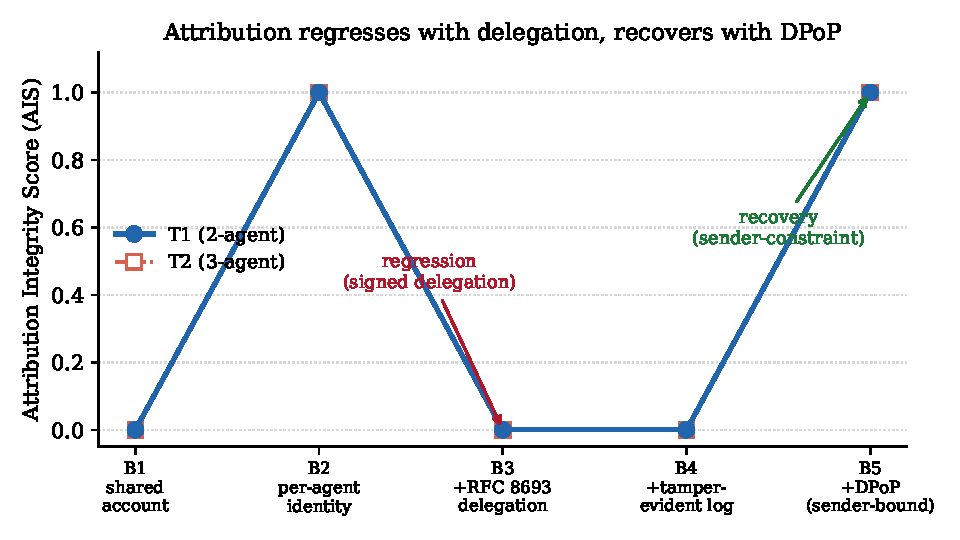
\includegraphics[width=0.92\linewidth]{fig_ais_curve}
\caption{The non-monotonic \ais{} curve, measured on both topologies. T1
(2-agent) and T2 (3-agent) land on identical points --- the gap does not
heal with chain depth (\S\ref{sec:topology}). Attribution regresses when
signed delegation is added (B3) and recovers when sender-constraint is added
(B5). Generated from the live harness.}
\label{fig:curve}
\end{figure}

\paragraph{Contributions.}
\begin{enumerate}[leftmargin=1.4em,itemsep=2pt]
  \item \textbf{A measured fix.} Baseline~5: \dpop{} sender-constrained
  tokens (RFC~9449) implemented by hand, recovering $\ais{}$ to $1.0$ on
  both topologies (\S\ref{sec:b5}, \S\ref{sec:results}).
  \item \textbf{A real measurement instrument.} A process-boundary recorder
  using OS process identity, removing v1's thread-name proxy and proven
  unspoofable by an in-process rename (\S\ref{sec:recorder}).
  \item \textbf{A second metric.} The Log Integrity Score (\lis{}), backed
  by a real hash-chained signed log, demonstrating that B4 is tamper-evident
  ($\lis{}=1.0$) yet still mis-attributing ($\ais{}=0.0$)
  (\S\ref{sec:lis}, \S\ref{sec:results}).
  \item \textbf{A second topology.} A 3-agent re-delegation chain (T2)
  showing the gap persists at depth~2 (\S\ref{sec:topology}).
  \item \textbf{Real confidence intervals.} A stochastic Bernoulli($p$)
  policy with Wilson 95\% intervals and adaptive sample-size escalation,
  showing the curve shape is invariant to attack frequency
  (\S\ref{sec:stochastic}, \S\ref{sec:results}).
  \item \textbf{Stronger pre-registration.} A SHA-256-locked threat model
  with a CI gate that fails the build on any edit, mechanizing v1's
  documentary pre-registration (\S\ref{sec:method}).
\end{enumerate}

\paragraph{Scope and honesty up front.}
v2 still concedes: only \dpop{} (not mutual-TLS, RFC~8705) is measured;
two topologies (linear only, no fan-in or cross-organization); scripted
deterministic agents (no LLM in the loop); and a synthetic Bernoulli policy
rather than real-world attack-frequency telemetry. These are deliberate
boundaries defended in \S\ref{sec:validity}.

% ===========================================================================
\section{Background and Relationship to v1}
\label{sec:background}
% ===========================================================================

We assume the v1 background~\cite{aegisv1}: RFC~8693's \code{act} claim and
its \S4.1 current-actor semantics; the confused-deputy lineage from
Hardy~\cite{hardy1988} through Clinejection~\cite{clinejection} and the CSA
confused-deputy note~\cite{csa2026}; the standards call from NIST
NCCoE~\cite{nist2026} and the OpenID Foundation~\cite{openid2026}; and the
positioning against \emph{The Misattribution Gap}~\cite{misattribution} and
SentinelAgent~\cite{sentinelagent}. This section adds only what v2 needs.

\subsection{Sender-constrained tokens: DPoP}
RFC~8693 inherits OAuth~2.0's default \emph{bearer} holder model: possession
of a token is sufficient to use it. \dpop{} (RFC~9449)~\cite{rfc9449} binds a
token to a key pair the legitimate holder controls. The token carries a
confirmation claim $\cnf = \{\jkt: t\}$ (RFC~7800~\cite{rfc7800}), where $t$
is the SHA-256 thumbprint (RFC~7638~\cite{rfc7638}) of the holder's public
key. On every request the holder presents a short-lived \emph{proof} JWT
signed by the private key and bound to the HTTP method and endpoint; the
resource verifies the proof and checks that the proof key's thumbprint
equals the token's $\jkt$. A party that does not hold the private key cannot
produce a valid proof, so it cannot wield the token. This is exactly the
binding v1 named as the hypothesized fix and did not measure; \S\ref{sec:b5}
measures it.

\subsection{What is inherited, and the one thing that moved}
The adversary model (gray-box; alert-content control only; no token forgery;
no process compromise), the attack mechanism (re-delegation misattribution,
Path~B), the delegation logic, the token-verification logic, and the
per-baseline credentials of Baselines~1--4 are inherited unchanged from
v1~\cite{aegisv1}. The four substrate modules (\code{auth/tokens.py},
\code{policy/scope\_map.py}, \code{harness/scorer.py} core,
\code{orchestrator/orchestrator.py}) are reused and extended, never rewritten,
so any \ais{} difference remains attributable to the configuration flag rather
than to incidental code differences.

One element of the \emph{execution substrate} did move, and we state it plainly
rather than let a reader infer it. In v1 each agent called \siem{} directly,
in its own thread and process. In v2 the agents are separate OS processes and
the tool call crosses the process boundary: the agent sends
\code{(command, target, credential, proof)} to the parent harness, which
invokes the recorder and \siem{} on its behalf (\S\ref{sec:recorder}). The tool
therefore executes inside the harness process. This is required for PID-based
ground truth and is neutral to the comparison --- the verification logic and
the presented credential are semantically identical to v1 on the B1--B4 path, and the claimed record still
derives solely from the presented token --- but it is a real change to the
substrate and we record it as a validity threat (\S\ref{sec:validity},
item~6).

% ===========================================================================
\section{Process-Boundary Ground Truth}
\label{sec:recorder}
% ===========================================================================

v1's recorder read \code{threading.current\_thread().name} as
\code{true\_actor} --- an honest proxy, but one a misbehaving agent could
spoof by renaming its thread. v1 excluded this by its adversary model (alert
text only, not agent code); a reviewer is nonetheless entitled to press on
it.

v2 removes the proxy. Agents run as \code{multiprocessing.Process} children
spawned by a kernel in the parent harness. The kernel registers the OS-assigned
PID $\to$ agent-name mapping \emph{at spawn, before the agent's user code
runs}, and resolves \code{true\_actor} from that registry. The agent's
tool-call message also self-reports its PID, but only so the kernel can
cross-check it and fail loud on a mismatch --- the resolved identity is always
the kernel's, never the message's. The recorder thus reads identity from the
kernel's spawn-time PID registry (the PID is OS-assigned), not from any
agent-supplied field. The
three independence axes from v1 are now \emph{real} rather than argued: a true
process boundary (a separate OS process), credential isolation (a per-agent
pipe whose child end alone crosses the boundary), and causal precedence
(register before serve).

\paragraph{Where the tool runs.} Because ground truth is the executing agent's
PID observed at the tool boundary, the tool call is mediated by the harness:
the agent body sends \code{(command, target, credential, proof)} over its
kernel pipe, and the parent harness runs the recorder and \siem{} for it,
attributing the call to the PID it registered for that pipe. The tool thus
executes in the harness process. Two consequences matter for validity.
\emph{First}, the agent's private \dpop{} key never crosses the boundary: the
call-time proof is signed \emph{inside} the agent process and only the signed
proof is sent (\S\ref{sec:b5}). \emph{Second}, nothing the tool verifies or
records changes --- the verification logic is semantically identical to v1 on the
B1--B4 path, the claimed
record derives solely from the presented token, and the true record solely from
the kernel PID --- so centralizing tool execution puts the tool on the same
side as the recorder without contaminating the claimed-vs-true comparison. We
nonetheless record this substrate change as a validity threat
(\S\ref{sec:validity}, item~6), as a production deployment would instead run
\siem{} as its own service and observe the caller's authenticated identity at
that service boundary --- the same construction, relocated.

\paragraph{Spoof resistance, measured.} A test agent that renames its thread
to \code{agent:enrich} --- the exact move that defeats the v1 recorder --- and
overwrites its process title obtains the \emph{same} attribution as a clean
run on every baseline: B2 stays $1.0$ and B3 stays $0.0$ with
\code{true\_actor} still observed as \code{contain}. An in-process rename
cannot move the call into another process, so PID-based attribution is
unmoved. The v1 thread-proxy caveat is retired, and v1's curve reproduces
exactly under the subprocess substrate (the regression gate).

% ===========================================================================
\section{Baseline 5: Sender-Constrained Tokens (DPoP)}
\label{sec:b5}
% ===========================================================================

\subsection{Mechanism}
Each agent is provisioned a \dpop{} key pair whose private half is used only
inside the agent process to sign proofs; the harness generates the keypair and
hands the agent its private key (as PKCS8 PEM) before the agent's code runs,
and only signed proofs --- never the private key --- cross back over the IPC
boundary (made precise in threat-model-v2.1 \S A5). A token minted for an agent
carries $\cnf=\{\jkt:t\}$ where
$t$ is the thumbprint of that agent's public key. The tool requires, on
every call: a valid proof JWT signed by the caller's key; equality of the
proof key's thumbprint and the token's $\jkt$; a fresh \code{jti} not in a
replay cache; and an \code{iat} within a 60-second window. The orchestrator,
when re-delegating, requires a proof from the receiving agent and binds the
new token's $\cnf$ to that agent's key --- so an agent cannot obtain a token
bound to a key it does not hold. Baselines~1--4 pass $\cnf=\textsc{none}$ and
are byte-for-byte the v1 path.

\subsection{Why it recovers the curve}
Under B1--B4, the token minted naming Enrich is an unbound bearer; Contain
lifts it and presents it, and nothing detects the substitution --- that lift
is the entire attack. Under B5 the token's $\jkt$ is \emph{Enrich's}
thumbprint, and Contain cannot sign a proof under Enrich's private key, so
the presentation is rejected before identity is resolved. To act legitimately
Contain must obtain its \emph{own} token --- bound to Contain's key, naming
Contain as current actor, via an execution-time re-exchange. The claimed
actor then tracks the executor, and attribution recovers. The replay cache
and \code{iat} window additionally reject a captured proof replayed by
another party.

\subsection{What the binding does and does not guarantee}
The orchestrator verifies \emph{possession}: the presenter holds the private
key whose thumbprint equals the token's \jkt{}. It does not, on its own,
verify that the name written into \actsub{} belongs to that key's holder. In
this benchmark the name--key correspondence is established two ways: by
construction (the harness mints the executor's token naming the executor and
bound to the executor's own freshly generated key), and at execution time (the
agent that signs the call-time proof the tool checks is the PID-registered
executor, \S\ref{sec:recorder}). The recovery to $\ais{}=1.0$ follows from the
executor wielding a token bound to its own key and naming itself. The distinct
variant ``an agent obtains a token \emph{naming a different actor} but bound to
its \emph{own} key'' is principal laundering --- a separate attack class v1 and
v2 backlog; defending it requires an orchestrator-side name~$\to$~registered-key
registry checked at mint time, named here as the production requirement. The
replay cache is a per-run, single-use \code{jti} set held in the parent harness
(no eviction is needed because each run is short and deterministic; a
production cache would bound retention to the proof window).

% ===========================================================================
\section{Hash-Chained Log and the Log Integrity Score}
\label{sec:lis}
% ===========================================================================

v1's Baseline~4 was attribution-only: it ran B3's code path, so B4~$=$~B3 by
construction. v2 builds the real artifact. Each B4 log entry carries
$\textsf{prev\_hash} = \textsf{SHA256}(\textsf{canonical}(\textsf{entry})
\,\|\, \textsf{prev\_hash})$, and the chain head is signed by an Ed25519
logger key held only by the parent harness --- no agent, the orchestrator, or
the tool holds it. A post-hoc rewrite is detectable two ways: the broken
chain link, and a head signature that no longer verifies.

\paragraph{The Log Integrity Score.} \lis{} is a metric distinct from \ais{}:
\[
\lis(B) = \frac{\#\,\text{tampered entries detected by chain verification}}
{\#\,\text{tampered entries}}.
\]
Under tamper injection (the reported experiments), a baseline with no
integrity artifact (B1--B3, B5) has no chain to verify, so a rewrite is
undetectable: \lis{} is $0.0$ \emph{by definition}
rather than undefined --- the question ``was the tamper detected?'' has a
well-defined answer (no), because a log with no integrity mechanism detects
nothing. For B4, every injected tamper is caught and $\lis{}=1.0$.

\paragraph{The load-bearing asymmetry.} \ais{} and \lis{} are orthogonal: a
baseline can score $\lis{}=1.0$ (tamper-evident) and $\ais{}=0.0$ (records the
wrong actor) simultaneously, which is exactly B4 (Figure~\ref{fig:lis}). The
wrong actor is committed upstream at minting, before any logging layer sees
the entry, so a perfect tamper-evident log faithfully preserves a wrong
record. This is v1's negative result, now backed by a real cryptographic
artifact rather than an asserted equality.

\begin{figure}[h]
\centering
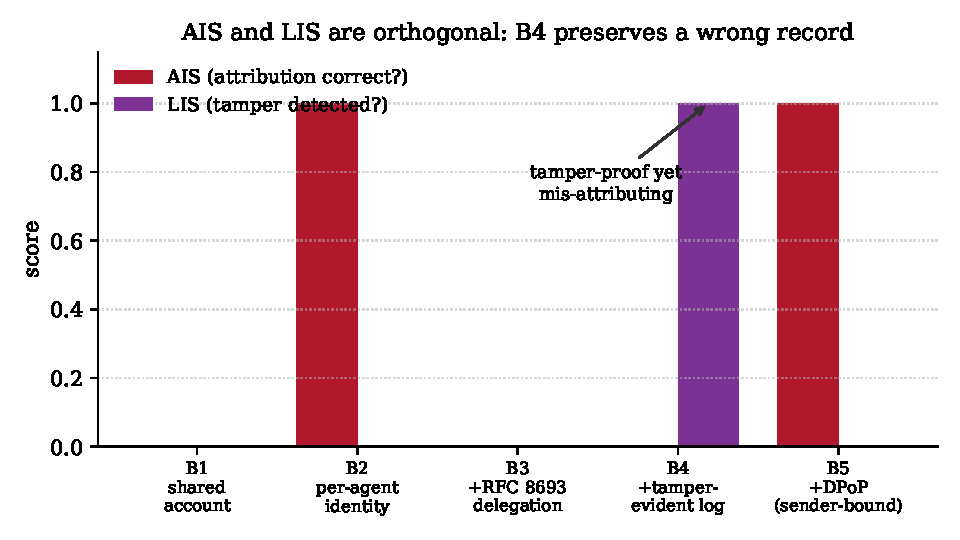
\includegraphics[width=0.92\linewidth]{fig_ais_lis}
\caption{\ais{} and \lis{} per baseline. Only B4 carries a hash-chained log,
so only B4 reaches $\lis{}=1.0$; yet B4's \ais{} is $0.0$ --- the tamper-evident
log preserves the wrong record. Generated from the live harness.}
\label{fig:lis}
\end{figure}

% ===========================================================================
\section{Topology T2: A Three-Agent Chain}
\label{sec:topology}
% ===========================================================================

v1's central conceded limitation was its single topology. v2 adds a second, T2:
a linear re-delegation chain \code{Agent-Enrich}~$\to$~%
\code{Agent-Investigator}~$\to$~\code{Agent-Contain}, two re-delegation hops.
Investigator is a mid-chain agent that receives Enrich's escalation, makes
its own correct judgment, and re-delegates containment onward; Contain still
executes. We choose a linear chain over a fan-in because linear isolates the
chain-\emph{depth} question without the concurrent-write log-ordering
confounds a fan-in would add.

The measured T2 curve is identical to T1
(Figure~\ref{fig:curve}; Table~\ref{tab:curve}). At B3/B4 on T2 the claimed
actor is the \emph{deepest} requester, Investigator, and the claimed
principal chain has grown a hop to
$[\code{investigator}, \code{enrich}, \code{analyst}]$ --- but the true actor
is still the executor, Contain. The gap therefore does not heal with depth;
it merely names a different non-executor. To foreclose an unregistered-choice
objection we pin the per-hop scope: the root token carries
\code{siem:read siem:write}, and \emph{every} re-delegation hop (Enrich, then
Investigator) narrows to \code{siem:write} --- it must, or Contain could not
execute \code{isolate\_host}. So at B3/B4 on T2 the claimed and true scope both
equal \code{siem:write} (scope \emph{matches}, as in T1); the defect is on
\code{actor} and \code{principal\_chain} only. Investigator's standing
``read-plus-correlate'' role does not change the scope of the containment
authority it re-delegates, and giving that token \code{siem:write} does not
prevent the misattribution (scope agreement is orthogonal to actor agreement).
B5 is topology-independent by construction: Contain's own bound token is rooted
directly at the analyst regardless of the attack path's depth, so B5 recovers
to $1.0$ on T2 as well. This moves the generalization claim from a structural
argument to a result shown on two topologies.

% ===========================================================================
\section{Stochastic Policy and Confidence Intervals}
\label{sec:stochastic}
% ===========================================================================

v1 reported $\ais{}\in\{0,1\}$ from a single canonical execution, so its
confidence intervals were degenerate. v2 makes the escalation policy
stochastic: Enrich escalates with probability $p\in\{0.1,0.5,0.9\}$, and we
run $N$ trials per (topology, baseline, $p$) cell, reporting a Wilson 95\%
interval on the resulting fraction. Cells whose interval half-width exceeds
$0.1$ at $N=100$ are automatically re-measured at $N=500$ (adaptive
escalation), which the low-frequency boundary cells (e.g.\ $p=0.1$) trigger.

\paragraph{An exact, not sampled, evaluation.} Per-action attribution
correctness is deterministic given (baseline, topology) --- v1's determinism
check proves a run is byte-reproducible, and the pre-registered claim is that
$p$ scales the \emph{number} of adversarial actions, not the per-action
correctness. We therefore evaluate the attack once per cell and draw $N$
seeded Bernoulli($p$) escalation events to form the denominator: re-running
the identical deterministic subprocess $N$ times would change nothing but
wall-clock. The randomness that matters --- which trials escalate --- is
seeded and reproducible, so the entire grid is a deterministic function of
one base seed. That seed is fixed and recorded in the artifact
(\code{base\_seed = 20260610}); the point predictions are seed-independent
(structural), while the exact interval bounds are a deterministic function of
the fixed seed, so the bounds reported below are reproducible exactly. We
report two denominators per cell (\S\ref{sec:results}): the adversarial-trigger
denominator (escalated trials, $\sim\!\mathrm{Bin}(N,p)$) and the
expanded/structural denominator (all $N$ re-delegated containments). The two
yield the same point \ais{} --- itself a manifestation of the structural nature
of the gap --- with the expanded denominator giving tighter intervals (its
size is always $N$).

% ===========================================================================
\section{Implementation}
\label{sec:impl}
% ===========================================================================

v2 reuses v1's four substrate modules unchanged in spirit and adds, over the
same package:
\begin{description}[leftmargin=1.6em,style=nextline,itemsep=2pt]
  \item[\code{auth/dpop.py}] The \dpop{} primitive: Ed25519 key pairs, proof
  JWT construction (\code{htm}/\code{htu}/\code{iat}/\code{jti}), RFC~7638
  thumbprints, and server-side proof verification (signature, binding,
  replay, freshness). A leaf module (Ed25519 only) so an agent subprocess can
  import it without the RSA-key-generating token module.
  \item[\code{harness/agent\_proc.py}, \code{agent\_bodies.py}] The
  process-boundary kernel and the bodies that run inside agent subprocesses;
  identity is the kernel's PID registry, cross-checked against the message's
  self-reported PID (fail loud on mismatch).
  \item[\code{harness/tamper\_log.py}] The hash-chained, logger-signed
  tamper-evident log; \code{verify} returns the indices of broken entries.
  \item[\code{harness/stochastic.py}] The Bernoulli($p$) sweep with Wilson
  intervals and adaptive sample-size escalation.
  \item[\code{topologies/}] T1 and T2 as data (a re-delegation hop list); the
  sweep builds tokens from the declaration, so adding a topology is adding
  data, not forking code.
  \item[\code{harness/scorer.py}] Extended with \code{score\_lis} alongside
  \code{score\_ais}; the \ais{} path is unchanged.
\end{description}
The token, scope-map, tool, and orchestrator modules gain only an optional,
defaulted $\cnf$/proof path that is inert on Baselines~1--4.

% ===========================================================================
\section{Experimental Methodology}
\label{sec:method}
% ===========================================================================

\paragraph{Pre-registration, now mechanized.} Every predicted value --- the
B1--B5 curve on both topologies, the \lis{} curve, and the stochastic
point predictions --- is committed in \code{threat-model-v2.md} before the
measuring code. v2 hardens v1's documentary pre-registration into a build
invariant: the threat model is hashed (SHA-256 over LF-normalized bytes) into
\code{threat-model-v2.sha256}, and a CI test recomputes the hash and fails the
build on any drift. The original file is never edited; clarifications and
amendments go in versioned files (\code{threat-model-v2.1.md}), each with its
own lock that the same CI test guards, so the amendment record is as
tamper-evident as the original. The v2.1 amendment records the disclosures
surfaced in external review (the tool-execution-context change, the precise
\dpop{} binding guarantee, the pinned per-hop scope, the fixed stochastic seed)
\emph{without altering any pre-registered prediction}. A contradicted
prediction is reported as a finding, not reconciled.

\paragraph{Determinism and reproducibility.}
Determinism is a checked property on both topologies: each baseline yields
byte-identical records across repeated runs under a fixed clock, and a
fault-injection test confirms the check catches a drifting clock. The
stochastic grid is reproducible from a single base seed. Figures are
generated from the live harness, so a plotted number cannot diverge from the
code. The suite is \textbf{74 v2 tests} plus the \textbf{59 frozen v1 tests};
both gates exit~0.

% ===========================================================================
\section{Results}
\label{sec:results}
% ===========================================================================

\subsection{The two curves}
The measured \ais{} curve reproduces the pre-registered prediction exactly on
both topologies (Table~\ref{tab:curve}, Figure~\ref{fig:curve}):
$B1{=}0.0,\,B2{=}1.0,\,B3{=}0.0,\,B4{=}0.0,\,B5{=}1.0$, identical for T1 and
T2. \code{is\_non\_monotonic} returns \code{True} on both. The B3 defect
breakdown confirms the mechanism rather than an accidental zero: on T1 the
claimed actor is \code{agent:enrich}, on T2 it is \code{agent:investigator}
(the deepest requester), and on both the true actor is \code{agent:contain},
with the \code{actor} and \code{principal\_chain} fields mismatched together
and \code{scope} matching. B5's recovery is likewise mechanistic: the lifted
token is rejected and the executor re-exchanges for its own bound token.

\subsection{Log integrity}
The \lis{} curve is $0.0$ for B1, B2, B3, B5 and $\mathbf{1.0}$ for B4
(Figure~\ref{fig:lis}): only the hash-chained log detects a post-hoc rewrite,
and it detects every one. B4's \ais{} remains $0.0$ in the same runs --- the
tamper-evident log preserves the wrong record. This is the §6.3 asymmetry
realized empirically.

\subsection{Stochastic confidence intervals}
The point \ais{} equals the pre-registered bit in every cell regardless of
$p$ and topology (\code{curve\_shape\_invariant} returns \code{True}); $p$
scales the denominator, not the correctness. Table~\ref{tab:stoch} shows
representative T1 cells under \emph{both} denominators of \S\ref{sec:stochastic}:
the adversarial-trigger denominator (escalated trials only) and the expanded
denominator (all $N$ re-delegated containments, threat-model-v2.md~\S4.3). The
two give identical point estimates --- confirming the threat-model~\S4.3
prediction that the misattribution is
latent in the re-delegation pattern, not created by the attacker --- while the
expanded denominator's intervals are tighter because its size is always $N$.
The low-frequency cells auto-escalate to $N=500$. Figure~\ref{fig:stoch} plots
the full grid.

\begin{table}[h]
\centering
\caption{Representative stochastic cells (topology T1), Wilson 95\% intervals
under both denominators. ``esc./$N$'' is the realized escalation count over the
trial count; $\dagger$ marks cells that auto-escalated from $N=100$ to $N=500$
because the $N=100$ adversarial half-width exceeded $0.1$. The point \ais{} is
identical under both denominators (threat-model~\S4.3); the expanded interval is tighter
(denominator $=N$). All values are reproducible from the fixed base seed
\code{20260610}.}
\label{tab:stoch}
\begin{tabular}{clcccc}
\toprule
\textbf{B} & \textbf{$p$} & \textbf{\ais{}} &
\textbf{adversarial 95\% CI} & \textbf{expanded 95\% CI} & \textbf{esc./$N$} \\
\midrule
B2 & 0.1 & 1.0 & $[0.935,\,1.000]$ & $[0.992,\,1.000]$ & 55/500$^\dagger$ \\
B2 & 0.5 & 1.0 & $[0.930,\,1.000]$ & $[0.963,\,1.000]$ & 51/100 \\
B2 & 0.9 & 1.0 & $[0.961,\,1.000]$ & $[0.963,\,1.000]$ & 95/100 \\
B3 & 0.5 & 0.0 & $[0.000,\,0.062]$ & $[0.000,\,0.037]$ & 58/100 \\
B5 & 0.1 & 1.0 & $[0.839,\,1.000]$ & $[0.963,\,1.000]$ & 20/100 \\
B5 & 0.9 & 1.0 & $[0.960,\,1.000]$ & $[0.963,\,1.000]$ & 92/100 \\
\bottomrule
\end{tabular}
\end{table}

\begin{figure}[h]
\centering
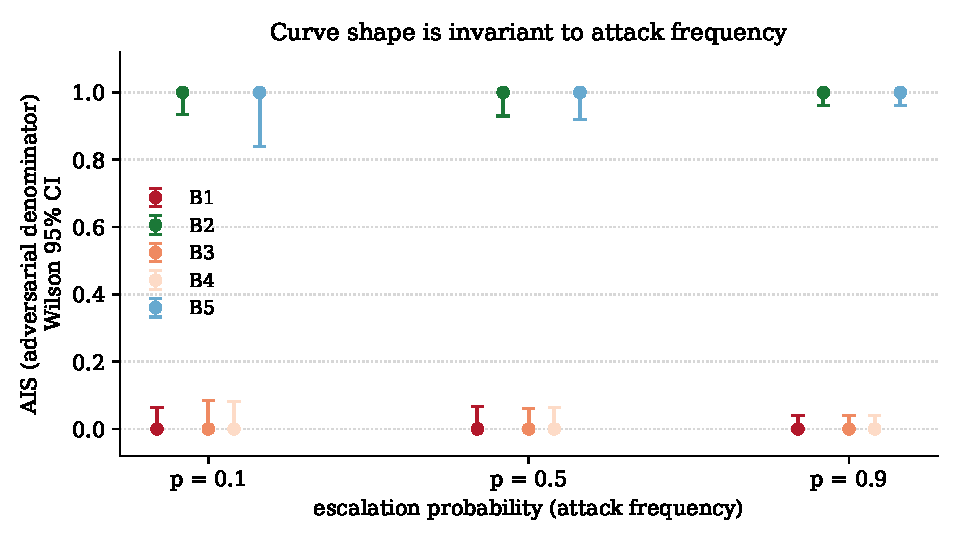
\includegraphics[width=0.92\linewidth]{fig_stochastic_ci}
\caption{Stochastic \ais{} with Wilson 95\% intervals across escalation
probability $p$ (topology T1, adversarial denominator). The point estimates
are flat across $p$ --- the curve shape is invariant to attack frequency ---
while the intervals tighten as $p$ (and the escalation count) grows.
Generated from the live harness.}
\label{fig:stoch}
\end{figure}

% ===========================================================================
\section{Discussion}
\label{sec:discussion}
% ===========================================================================

\paragraph{Sender-constraint is the layer that closes the gap.}
v1 named \dpop{} as the hypothesized fix and declined to claim it worked
without measuring it. v2 measures it: B5 recovers \ais{} to $1.0$ on both
topologies. The mechanism is precise --- the lift that constitutes the attack
is rejected because Contain cannot prove possession of Enrich's key, forcing
an execution-time re-exchange that names the executor. This converts v1's
``named fix'' into a measured one and localizes the missing layer exactly: not
``log a different field'' (there is no such field) but ``bind the token to the
executor's key and require an execution-time re-exchange that names the
executor.''

\paragraph{The robustness changes strengthen, not weaken, the v1 finding.}
A skeptic could have attributed v1's result to its thread-name proxy, its
stub Baseline~4, its single topology, or its degenerate intervals. v2 removes
all four: a real process boundary (spoof-resistant), a real hash-chained log
(B4 \lis{}$=1.0$ yet \ais{}$=0.0$), a second topology (gap persists at
depth~2), and real Wilson intervals (shape invariant across $p$). Each could
have contradicted v1; none did. The gap survives every hardening.

\paragraph{Tamper-evidence and chain depth are orthogonal to attribution.}
The \lis{} result makes concrete what v1 argued: a cryptographically perfect
audit log can certify the integrity of a wrong record. The T2 result makes
concrete that adding hops does not help: each additional requester is one more
non-executor the log can name. Both confirm that the only axis that moves
\ais{} is whether the recorded identity is bound to the executor --- which is
what B2 (authenticator = executor) and B5 (sender-constraint) achieve and
B1/B3/B4 do not.

% ===========================================================================
\section{Limitations and Validity Threats}
\label{sec:validity}
% ===========================================================================

\begin{enumerate}[leftmargin=1.6em,itemsep=3pt]
  \item \textbf{DPoP only, not mutual-TLS.} v2 measures sender-constraint via
  \dpop{} (RFC~9449). Mutual-TLS-bound tokens (RFC~8705) are a second
  standardized binding; they require TLS infrastructure and are predicted to
  behave identically (both close the unbound-bearer gap). Measuring them is a
  v3 ``Baseline~5b.''
  \item \textbf{Two topologies, linear only.} T1 and T2 are linear chains.
  Fan-in (two agents re-delegating into one executor) and cross-organization
  delegation each add confounds --- concurrent-write log ordering, multiple
  trust domains --- and are deferred to v3.
  \item \textbf{Scripted agents.} As in v1, the agents are deterministic
  scripts, which isolates the delegation layer from model behavior but does
  not measure interaction with imperfect LLM decisions. An optional LLM
  adapter is deferred to avoid an API-key dependency in the reproducible core.
  \item \textbf{Synthetic policy.} The Bernoulli($p$) escalation is a
  controlled synthetic policy, not real-world attack-frequency telemetry.
  Real distributions await an industry partner.
  \item \textbf{Independence by construction.} The recorder's independence is
  now a real process boundary rather than a thread proxy, but it is still
  established by construction and property-based testing, not formal
  verification.
  \item \textbf{Tool execution is centralized in the harness.} To observe the
  executing agent's PID at the tool boundary (\S\ref{sec:recorder}), the agent
  sends its tool call over IPC and the parent harness runs \siem{} for it, so
  the tool executes in the harness process rather than the agent's --- a change
  from v1, where the agent's own thread called the tool. We argue this does not
  affect the result: the attack's injection, minting, and hand-off all precede
  the tool call; the tool's verification logic and the presented credential are
  semantically identical to v1 on the B1--B4 path; the agent's \dpop{} private key never crosses the
  boundary (the proof is signed in the agent process); and the claimed record
  still derives solely from the presented token while the true record derives
  solely from the kernel PID. What moved is the host process of an unchanged
  computation. A production deployment would run \siem{} as its own service and
  authenticate the caller at that service boundary --- the same construction,
  relocated. This substrate change is also recorded in the locked threat-model
  amendment (\code{threat-model-v2.1.md} §A1).
\end{enumerate}

% ===========================================================================
\section{Future Work}
\label{sec:future}
% ===========================================================================

\begin{itemize}[leftmargin=1.4em,itemsep=2pt]
  \item \textbf{Baseline 5b --- mutual-TLS.} Measure RFC~8705 certificate-bound
  tokens alongside \dpop{}; confirm the predicted equivalence.
  \item \textbf{Fan-in and cross-organization topologies.} Move from two
  linear topologies to aggregation and multi-trust-domain delegation.
  \item \textbf{LLM-in-the-loop.} An optional adapter that plugs a frontier
  model in as Enrich or Contain, demonstrating the gap holds when the
  escalating agent is a real LLM, as an appendix demonstration outside the
  reproducible core.
  \item \textbf{Real telemetry.} Replace the synthetic Bernoulli policy with
  observed escalation frequencies from a partner SOC deployment.
  \item \textbf{Other sibling-impersonation variants.} Delegation forgery,
  scope-attenuation bypass, principal laundering --- each a distinct mode.
\end{itemize}

% ===========================================================================
\section{Conclusion}
\label{sec:conclusion}
% ===========================================================================

AEGIS-AT v1 showed that RFC~8693 delegation can make multi-agent audit
attribution worse, not better. v2 asked whether the standardized fix recovers
it and whether the finding survives hardening. It does and it does:
sender-constrained tokens (\dpop{}) recover the Attribution Integrity Score to
$1.0$ at Baseline~5, while a real process boundary, a real hash-chained log,
a second topology, and real confidence intervals each leave the non-monotonic
curve standing. The Log Integrity Score makes the negative result concrete --- a
tamper-evident log of the wrong actor --- and the three-agent chain shows the gap
does not heal with depth. The attribution gap is structural; tamper-evidence
and chain depth are orthogonal to it; and binding the token to its holder is
the layer that closes it. As standards bodies make RFC~8693 the backbone of AI
agent non-repudiation, v2 is a concrete demonstration of both the gap and the
specific standardized layer that closes it.

% ===========================================================================
\section*{Reproducibility and Artifact Availability}
\addcontentsline{toc}{section}{Reproducibility and Artifact Availability}
% ===========================================================================
The complete v2 benchmark --- the SHA-256-locked threat model, the new and
extended modules, the harness, and 74 tests --- is released alongside the
frozen v1 artifact (tag \code{v1.0.0}). Code is licensed Apache-2.0;
documentation CC~BY~4.0. Every \ais{}, \lis{}, and stochastic value is
asserted in the test suite against a prediction locked before the measuring
code was written, and the figures regenerate from the live harness via
\code{python Documents/Paper/figures/make\_figures.py}. The pipeline
reproduces in seconds.

% ===========================================================================
\begin{thebibliography}{99}
\addcontentsline{toc}{section}{References}

\bibitem{aegisv1} R.~Singh, \emph{AEGIS-AT: Measuring Attribution Integrity
Under Sibling Impersonation in Multi-Agent Delegation} (v1), 2026. Frozen
artifact, tag \code{v1.0.0}.
\url{https://github.com/rahulsingh1397/AEGIS-AT}.

\bibitem{rfc8693} M.~Jones, A.~Nadalin, B.~Campbell, J.~Bradley, and C.~Mortimore,
\emph{OAuth 2.0 Token Exchange}, RFC~8693, IETF, January 2020.
\url{https://www.rfc-editor.org/rfc/rfc8693}.

\bibitem{rfc9449} D.~Fett, B.~Campbell, J.~Bradley, T.~Lodderstedt, M.~Jones, and
D.~Waite, \emph{OAuth 2.0 Demonstrating Proof of Possession (DPoP)}, RFC~9449,
IETF, September 2023. \url{https://www.rfc-editor.org/rfc/rfc9449}.

\bibitem{rfc8705} B.~Campbell, J.~Bradley, N.~Sakimura, and T.~Lodderstedt,
\emph{OAuth 2.0 Mutual-TLS Client Authentication and Certificate-Bound Access
Tokens}, RFC~8705, IETF, February 2020.
\url{https://www.rfc-editor.org/rfc/rfc8705}.

\bibitem{rfc7800} M.~Jones, J.~Bradley, and H.~Tschofenig, \emph{Proof-of-Possession
Key Semantics for JSON Web Tokens (JWTs)}, RFC~7800, IETF, April 2016.
\url{https://www.rfc-editor.org/rfc/rfc7800}.

\bibitem{rfc7638} M.~Jones and N.~Sakimura, \emph{JSON Web Key (JWK) Thumbprint},
RFC~7638, IETF, September 2015. \url{https://www.rfc-editor.org/rfc/rfc7638}.

\bibitem{nist2026} H.~Booth, W.~Fisher, R.~Galluzzo, and J.~Roberts,
\emph{Accelerating the Adoption of Software and Artificial Intelligence Agent
Identity and Authorization}, NIST NCCoE Concept Paper (Initial Public Draft),
February~5, 2026.
\url{https://www.nccoe.nist.gov/publications/other/accelerating-adoption-software-and-ai-agent-identity-and-authorization-concept}.

\bibitem{openid2026} OpenID Foundation, \emph{OIDF Responds to NIST on AI Agent
Security}, March~11, 2026.
\url{https://openid.net/oidf-responds-to-nist-on-ai-agent-security/}.

\bibitem{csa2026} Cloud Security Alliance AI Safety Initiative, \emph{Confused
Deputy Attacks on Autonomous AI Agents} (Research Note), March~23, 2026.
\url{https://labs.cloudsecurityalliance.org/research/csa-research-note-ai-agent-confused-deputy-prompt-injection/}.

\bibitem{clinejection} Snyk, \emph{How ``Clinejection'' Turned an AI Bot into a
Supply Chain Attack}, February 2026.
\url{https://snyk.io/blog/cline-supply-chain-attack-prompt-injection-github-actions/}.

\bibitem{misattribution} T.~Ahad, I.~Hossain, M.~J.~Alam, S.~Puppala,
S.~B.~Alam, and S.~Talukder, \emph{The Misattribution Gap: When Memory Poisoning
Looks Like Model Failure in Agentic AI Systems}, arXiv:2605.22842, May 2026.
\url{https://arxiv.org/abs/2605.22842}.

\bibitem{hardy1988} N.~Hardy, \emph{The Confused Deputy (or why capabilities might
have been invented)}, ACM SIGOPS Operating Systems Review, 22(4), 1988.

\bibitem{sentinelagent} K.~S.~R.~Patil, \emph{SentinelAgent: Intent-Verified
Delegation Chains for Securing Federal Multi-Agent AI Systems}, arXiv:2604.02767,
April 2026. \url{https://arxiv.org/abs/2604.02767}.

\bibitem{agenticjwt} A.~Goswami, \emph{Agentic JWT: Secure Delegation for Agentic AI},
arXiv:2509.13597, September 2025. \url{https://arxiv.org/abs/2509.13597}.

\end{thebibliography}

\end{document}
